\usepackage{tikz}
\usetikzlibrary{calc}
\usetikzlibrary{fadings}
\usetikzlibrary{decorations.markings}
\usetikzlibrary{arrows.meta}
\usetikzlibrary{backgrounds}

% colors for "face" domain walls
\definecolor{DarkerBlue}{HTML}{2C3645}
\definecolor{LighterBlue}{HTML}{87BDEF}

%%%%%%%%%%%%%%%%%%%%%%%%%%%%%%%%%%%%%%%%%%%%%%%%%%%%%%%%%%%%%%%
%        Notation for spins on edges and vertices             %
%%%%%%%%%%%%%%%%%%%%%%%%%%%%%%%%%%%%%%%%%%%%%%%%%%%%%%%%%%%%%%%

\newcommand{\redcirc}[2]{\fill   [BrickRed]    ({#1}, {#2}) circle(0.6ex);}
\newcommand{\greencirc}[2]{\fill [ForestGreen] ({#1}, {#2}) circle(0.6ex);}
\newcommand{\bluecirc}[2]{\fill  [RoyalBlue]   ({#1}, {#2}) circle(0.6ex);}

\newcommand{\redsquare}[2]{%
\fill   [BrickRed]   ({#1ex-.5ex}, {#2ex-.5ex}) rectangle({#1ex+.5ex}, {#2ex+.5ex});}
\newcommand{\greensquare}[2]{%
\fill [ForestGreen]  ({#1ex-.5ex}, {#2ex-.5ex}) rectangle({#1ex+.5ex}, {#2ex+.5ex});}
\newcommand{\bluesquare}[2]{%
\fill  [RoyalBlue]   ({#1ex-.5ex}, {#2ex-.5ex}) rectangle({#1ex+.5ex}, {#2ex+.5ex});}

\DeclareRobustCommand{\dualRcirc}[2]{%
\draw [thick, BrickRed] ({#1}, {#2 -1.2ex}) to ({#1}, {#2 + 1.2ex});%
\fill [BrickRed] ({#1}, {#2}) circle(0.6ex);%
}
\DeclareRobustCommand{\dualGcirc}[2]{%
\draw [thick, ForestGreen] ({#1}, {#2 -1.2ex}) to ({#1}, {#2 + 1.2ex});%
\fill [ForestGreen] ({#1}, {#2}) circle(0.6ex);%
}
\DeclareRobustCommand{\dualBcirc}[2]{%
\draw [thick, RoyalBlue] ({#1}, {#2 -1.2ex}) to ({#1}, {#2 + 1.2ex});%
\fill  [RoyalBlue]   ({#1}, {#2}) circle(0.6ex);%
}

\newcommand{\Redge}[2]{\fill [BrickRed]    ({#1}, {#2}) circle(0.5ex);}
\newcommand{\Gedge}[2]{\fill [ForestGreen] ({#1}, {#2}) circle(0.5ex);}
\newcommand{\Bedge}[2]{\fill [RoyalBlue]   ({#1}, {#2}) circle(0.5ex);}

\newcommand{\redket}{\ket{\kern1pt\tikz[baseline={(0,-0.1)}]\redsquare{0}{0};\kern1pt}}
\newcommand{\greenket}{\ket{\kern1pt\tikz[baseline={(0,-0.1)}]\greensquare{0}{0};\kern1pt}}
\newcommand{\blueket}{\ket{\kern1pt\tikz[baseline={(0,-0.1)}]\bluesquare{0}{0};\kern1pt}}

\newcommand{\dualRket}{\ket{\kern1pt\tikz[baseline={(0,-0.12)}]\dualRcirc{0}{0};\kern1pt}}
\newcommand{\dualGket}{\ket{\kern1pt\tikz[baseline={(0,-0.12)}]\dualGcirc{0}{0};\kern1pt}}
\newcommand{\dualBket}{\ket{\kern1pt\tikz[baseline={(0,-0.12)}]\dualBcirc{0}{0};\kern1pt}}

%%%%%%%%%%%%%%%%%%%%%%%%%%%%%%%%%%%%%%%%%%%%%%%%%%%%%%%%%%%%%%%
%       Useful "states" (generated using ketdraw.py)          %
%%%%%%%%%%%%%%%%%%%%%%%%%%%%%%%%%%%%%%%%%%%%%%%%%%%%%%%%%%%%%%%

\newcommand{\redpair}{\left\lvert\kern1pt%
    
\begin{tikzpicture}[baseline={(0,-0.12)},x=1ex, y=1ex]%
        \dualRcirc{0}{0};
        \dualRcirc{2.4}{0};
    \end{tikzpicture}\kern1pt\right\rangle}

\newcommand{\RedPairJoin}{\left\lvert\kern1pt%
    
\begin{tikzpicture}[baseline={(0,-0.12)},x=1ex, y=1ex]%
        \draw[BrickRed, thick, double] (0, 0)--(2.4, 0);
        \redcirc{0}{0};
        \redcirc{2.4}{0};
    \end{tikzpicture}\kern1pt\right\rangle}

\newcommand{\BGket}{\left\lvert\kern1pt%
    
\begin{tikzpicture}%
    \bluesquare{0.0}{0};%
    \greensquare{2.4}{0};%
    \end{tikzpicture}\kern1pt\right\rangle
}

\newcommand{\RGRket}{\left\lvert\kern1pt%
    
\begin{tikzpicture}[baseline={(0,-0.1)}]%
        \redsquare{0}{0};%
        \greensquare{2.4}{0};%
        \redsquare{4.8}{0};%
    \end{tikzpicture}\kern1pt\right\rangle}

\newcommand{\BRGket}{\left\lvert\kern1pt%
    
\begin{tikzpicture}%
        \fill[RoyalBlue] circle(0.6ex);%
        \fill[BrickRed] (2.4ex, 0) circle(0.6ex);%
        \fill[ForestGreen] (4.8ex, 0) circle(0.6ex);%
    \end{tikzpicture}\kern1pt\right\rangle}

\newcommand{\BGRGket}{\left\lvert\kern1pt%
    
\begin{tikzpicture}%
    \bluesquare{0.0}{0};%
    \greensquare{2.4}{0};%
    \redsquare{4.8}{0};%
    \greensquare{7.2}{0};%
    \end{tikzpicture}\kern1pt\right\rangle
}

\newcommand{\BGBGket}{\left\lvert\kern1pt%
    
\begin{tikzpicture}%
    \bluesquare{0.0}{0};%
    \greensquare{2.4}{0};%
    \bluesquare{4.8}{0};%
    \greensquare{7.199999999999999}{0};%
    \end{tikzpicture}\kern1pt\right\rangle
}

\newcommand{\BBBGket}{\left\lvert\kern1pt%
    
\begin{tikzpicture}%
    \bluesquare{0.0}{0};%
    \bluesquare{2.4}{0};%
    \bluesquare{4.8}{0};%
    \greensquare{7.199999999999999}{0};%
    \end{tikzpicture}\kern1pt\right\rangle
}

\newcommand{\BRGRGket}{\left\lvert\kern1pt%
    
\begin{tikzpicture}%
        \fill[RoyalBlue] circle(0.6ex);%
        \fill[BrickRed] (2.4ex, 0) circle(0.6ex);%
        \fill[ForestGreen] (4.8ex, 0) circle(0.6ex);%
        \fill[BrickRed] (7.2ex, 0) circle(0.6ex);%
        \fill[ForestGreen] (9.6ex, 0) circle(0.6ex);%
    \end{tikzpicture}\kern1pt\right\rangle}

\newcommand{\BRBRGket}{\left\lvert\kern1pt%
    
\begin{tikzpicture}%
        \fill[RoyalBlue] circle(0.6ex);%
        \fill[BrickRed] (2.4ex, 0) circle(0.6ex);%
        \fill[RoyalBlue] (4.8ex, 0) circle(0.6ex);%
        \fill[BrickRed] (7.2ex, 0) circle(0.6ex);%
        \fill[ForestGreen] (9.6ex, 0) circle(0.6ex);%
    \end{tikzpicture}\kern1pt\right\rangle}

\newcommand{\BGBRGket}{\left\lvert\kern1pt%
    
\begin{tikzpicture}%
        \fill[RoyalBlue] circle(0.6ex);%
        \fill[ForestGreen] (2.4ex, 0) circle(0.6ex);%
        \fill[RoyalBlue] (4.8ex, 0) circle(0.6ex);%
        \fill[BrickRed] (7.2ex, 0) circle(0.6ex);%
        \fill[ForestGreen] (9.6ex, 0) circle(0.6ex);%
    \end{tikzpicture}\kern1pt\right\rangle}

\newcommand{\RBsite}{\Big\lvert\kern0pt%
    
\begin{tikzpicture}[baseline={(0,-0.12)}]%
        \draw [semithick] (-1.2ex, 1.2ex)--(1.2ex, 1.2ex);%
        \draw [semithick] (-1.2ex, -1.2ex)--(1.2ex, -1.2ex);%
        \draw [semithick] (1.2ex, -1.2ex)--(1.2ex, 1.2ex);%
        \draw [semithick] (-1.2ex, -1.2ex)--(-1.2ex, 1.2ex);%
        \draw [BrickRed, thick, rounded corners=0.65ex] (-2.4ex, 0)--(0, 0)--(0, 2.4ex);%
        \draw [RoyalBlue, thick, rounded corners=0.65ex] (2.4ex, 0)--(0, 0)--(0, -2.4ex);%
        \fill[BrickRed] (-1.2ex, 0) circle(0.5ex);%
        \fill[RoyalBlue] (1.2ex, 0) circle(0.5ex);%
        \fill[BrickRed] (0, 1.2ex) circle(0.5ex);%
        \fill[RoyalBlue] (0, -1.2ex) circle(0.5ex);%
    \end{tikzpicture}\kern-2pt\Big\rangle}

\newcommand{\BGsite}{\Big\lvert\kern0pt%
    
\begin{tikzpicture}[baseline={(0,-0.12)}]%
        \draw [semithick] (-1.2ex, 1.2ex)--(1.2ex, 1.2ex);%
        \draw [semithick] (-1.2ex, -1.2ex)--(1.2ex, -1.2ex);%
        \draw [semithick] (1.2ex, -1.2ex)--(1.2ex, 1.2ex);%
        \draw [semithick] (-1.2ex, -1.2ex)--(-1.2ex, 1.2ex);%
        \draw [ForestGreen, thick, rounded corners=0.65ex] (-2.4ex, 0)--(0, 0)--(0, -2.4ex);%
        \draw [RoyalBlue, thick, rounded corners=0.65ex] (2.4ex, 0)--(0, 0)--(0, 2.4ex);%
        \fill[ForestGreen] (-1.2ex, 0) circle(0.5ex);%
        \fill[RoyalBlue] (1.2ex, 0) circle(0.5ex);%
        \fill[RoyalBlue] (0, 1.2ex) circle(0.5ex);%
        \fill[ForestGreen] (0, -1.2ex) circle(0.5ex);%
    \end{tikzpicture}\kern-2pt\Big\rangle}

\newcommand{\RQuad}{\Bigg\lvert\kern0pt%
    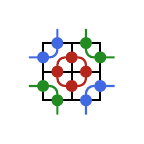
\begin{tikzpicture}[baseline={(0,-0.12)}]%
        \draw [thick, RoyalBlue, rounded corners=0.65ex] (-3.6ex, 1.2ex)--++(2.4ex, 0)--++(0, 2.4ex);
        \draw [thick, RoyalBlue, rounded corners=0.65ex] (3.6ex, -1.2ex)--++(-2.4ex, 0)--++(0, -2.4ex);
        \draw [thick, ForestGreen, rounded corners=0.65ex] (-3.6ex, -1.2ex)--++(2.4ex, 0)--++(0, -2.4ex);
        \draw [thick, ForestGreen, rounded corners=0.65ex] (3.6ex, 1.2ex)--++(-2.4ex, 0)--++(0, 2.4ex);
        \draw [thick, BrickRed, rounded corners=0.65ex] (-1.2ex, 0)--++(0, 1.2ex)--++(2.4ex, 0)--++(0, -2.4ex)--++(-2.4ex, 0)--(-1.2ex, 0);
        \draw [semithick] (-2.4ex, -2.4ex) rectangle (2.4ex, 2.4ex);%
        \draw [semithick] (0, -2.4ex) rectangle (0, 2.4ex);%
        \draw [semithick] (-2.4ex, 0) rectangle (2.4ex, 0);%
        %
        \fill [BrickRed] (-1.2ex, 0) circle(0.5ex);%
        \fill [BrickRed] (1.2ex, 0) circle(0.5ex);%
        \fill [BrickRed] (0, -1.2ex) circle(0.5ex);%
        \fill [BrickRed] (0, 1.2ex) circle(0.5ex);%
        \fill [RoyalBlue] (-1.2ex, 2.4ex) circle(0.5ex);%
        \fill [ForestGreen] (1.2ex, 2.4ex) circle(0.5ex);%
        \fill [RoyalBlue] (-2.4ex, 1.2ex) circle(0.5ex);%
        \fill [ForestGreen] (2.4ex, 1.2ex) circle(0.5ex);%
        \fill [ForestGreen] (-1.2ex, -2.4ex) circle(0.5ex);%
        \fill [RoyalBlue] (1.2ex, -2.4ex) circle(0.5ex);%
        \fill [ForestGreen] (-2.4ex, -1.2ex) circle(0.5ex);%
        \fill [RoyalBlue] (2.4ex, -1.2ex) circle(0.5ex);%
    \end{tikzpicture}\kern0pt\Bigg\rangle}

\newcommand{\BQuad}{\Bigg\lvert\kern0pt%
    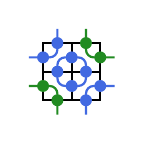
\begin{tikzpicture}[baseline={(0,-0.12)}]%
        \draw [thick, RoyalBlue, rounded corners=0.65ex] (-3.6ex, 1.2ex)--++(2.4ex, 0)--++(0, 2.4ex);
        \draw [thick, RoyalBlue, rounded corners=0.65ex] (3.6ex, -1.2ex)--++(-2.4ex, 0)--++(0, -2.4ex);
        \draw [thick, ForestGreen, rounded corners=0.65ex] (-3.6ex, -1.2ex)--++(2.4ex, 0)--++(0, -2.4ex);
        \draw [thick, ForestGreen, rounded corners=0.65ex] (3.6ex, 1.2ex)--++(-2.4ex, 0)--++(0, 2.4ex);
        \draw [thick, RoyalBlue, rounded corners=0.65ex] (-1.2ex, 0)--++(0, 1.2ex)--++(2.4ex, 0)--++(0, -2.4ex)--++(-2.4ex, 0)--(-1.2ex, 0);
        \draw [semithick] (-2.4ex, -2.4ex) rectangle (2.4ex, 2.4ex);%
        \draw [semithick] (0, -2.4ex) rectangle (0, 2.4ex);%
        \draw [semithick] (-2.4ex, 0) rectangle (2.4ex, 0);%
        %
        \fill [RoyalBlue] (-1.2ex, 0) circle(0.5ex);%
        \fill [RoyalBlue] (1.2ex, 0) circle(0.5ex);%
        \fill [RoyalBlue] (0, -1.2ex) circle(0.5ex);%
        \fill [RoyalBlue] (0, 1.2ex) circle(0.5ex);%
        \fill [RoyalBlue] (-1.2ex, 2.4ex) circle(0.5ex);%
        \fill [ForestGreen] (1.2ex, 2.4ex) circle(0.5ex);%
        \fill [RoyalBlue] (-2.4ex, 1.2ex) circle(0.5ex);%
        \fill [ForestGreen] (2.4ex, 1.2ex) circle(0.5ex);%
        \fill [ForestGreen] (-1.2ex, -2.4ex) circle(0.5ex);%
        \fill [RoyalBlue] (1.2ex, -2.4ex) circle(0.5ex);%
        \fill [ForestGreen] (-2.4ex, -1.2ex) circle(0.5ex);%
        \fill [RoyalBlue] (2.4ex, -1.2ex) circle(0.5ex);%
    \end{tikzpicture}\kern0pt\Bigg\rangle}

\newcommand{\BQuadAlt}{\Bigg\lvert\kern0pt%
    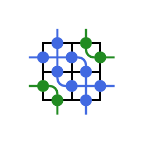
\begin{tikzpicture}[baseline={(0,-0.12)}]%
        \draw [thick, RoyalBlue, rounded corners=0.65ex] (-3.6ex, 1.2ex)--++(4.8ex, 0)--++(0, -4.8ex);
        \draw [thick, RoyalBlue, rounded corners=0.65ex] (3.6ex, -1.2ex)--++(-4.8ex, 0)--++(0, 4.8ex);
        \draw [thick, ForestGreen, rounded corners=0.65ex] (-3.6ex, -1.2ex)--++(2.4ex, 0)--++(0, -2.4ex);
        \draw [thick, ForestGreen, rounded corners=0.65ex] (3.6ex, 1.2ex)--++(-2.4ex, 0)--++(0, 2.4ex);
        \draw [semithick] (-2.4ex, -2.4ex) rectangle (2.4ex, 2.4ex);%
        \draw [semithick] (0, -2.4ex) rectangle (0, 2.4ex);%
        \draw [semithick] (-2.4ex, 0) rectangle (2.4ex, 0);%
        %
        \fill [RoyalBlue] (-1.2ex, 0) circle(0.5ex);%
        \fill [RoyalBlue] (1.2ex, 0) circle(0.5ex);%
        \fill [RoyalBlue] (0, -1.2ex) circle(0.5ex);%
        \fill [RoyalBlue] (0, 1.2ex) circle(0.5ex);%
        \fill [RoyalBlue] (-1.2ex, 2.4ex) circle(0.5ex);%
        \fill [ForestGreen] (1.2ex, 2.4ex) circle(0.5ex);%
        \fill [RoyalBlue] (-2.4ex, 1.2ex) circle(0.5ex);%
        \fill [ForestGreen] (2.4ex, 1.2ex) circle(0.5ex);%
        \fill [ForestGreen] (-1.2ex, -2.4ex) circle(0.5ex);%
        \fill [RoyalBlue] (1.2ex, -2.4ex) circle(0.5ex);%
        \fill [ForestGreen] (-2.4ex, -1.2ex) circle(0.5ex);%
        \fill [RoyalBlue] (2.4ex, -1.2ex) circle(0.5ex);%
    \end{tikzpicture}\kern0pt\Bigg\rangle}

\newcommand{\RBRBsite}{\Big\lvert\kern0pt%
    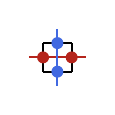
\begin{tikzpicture}[baseline={(0,-0.12)}]%
        \draw [semithick] (-1.2ex, 1.2ex)--(1.2ex, 1.2ex);%
        \draw [semithick] (-1.2ex, -1.2ex)--(1.2ex, -1.2ex);%
        \draw [semithick] (1.2ex, -1.2ex)--(1.2ex, 1.2ex);%
        \draw [semithick] (-1.2ex, -1.2ex)--(-1.2ex, 1.2ex);%
        \fill[BrickRed] (-1.2ex, 0) circle(0.5ex);%
        \fill[BrickRed] (1.2ex, 0) circle(0.5ex);%
        \fill[RoyalBlue] (0, 1.2ex) circle(0.5ex);%
        \fill[RoyalBlue] (0, -1.2ex) circle(0.5ex);%
        \draw [BrickRed, thick] (-2.4ex, 0)--(0, 0)--(2.4ex, 0);
        \draw [RoyalBlue, thick] (0, 2.4ex)--(0, 0)--(0, -2.4ex);
        %\fill[white] (0, 0) circle(0.5ex);%
        %\fill[black] (0, 0) circle(0.3ex);%
    \end{tikzpicture}\kern-2pt\Big\rangle}

\newcommand{\GBsite}{\Big\lvert\kern0pt%
    
\begin{tikzpicture}[baseline={(0,-0.12)}]%
        \draw [semithick] (-1.2ex, -1.2ex) rectangle (1.2ex, 1.2ex);%
        \fill[ForestGreen] (-1.2ex, 0) circle(0.5ex);%
        \fill[RoyalBlue] (1.2ex, 0) circle(0.5ex);%
        \fill[ForestGreen] (0, 1.2ex) circle(0.5ex);%
        \fill[RoyalBlue] (0, -1.2ex) circle(0.5ex);%
        \draw [ForestGreen, thick, rounded corners=0.65ex] (-2.4ex, 0)--(0, 0)--(0, 2.4ex);
        \draw [RoyalBlue, thick, rounded corners=0.65ex] (2.4ex, 0)--(0, 0)--(0, -2.4ex);
    \end{tikzpicture}\kern-2pt\Big\rangle}

\newcommand{\RRsite}{\Big\lvert\kern0pt%
    
\begin{tikzpicture}[baseline={(0,-0.12)}]%
        \draw [semithick] (-1.2ex, -1.2ex) rectangle (1.2ex, 1.2ex);%
        %\draw [BrickRed, thick, rounded corners=0.65ex] (-2.4ex, 0)--(0, 0)--(0, 2.4ex);%
        %\draw [BrickRed, thick, rounded corners=0.65ex] (2.4ex, 0)--(0, 0)--(0, -2.4ex);%
        \draw [BrickRed, thick] (-2.4ex, 0)--(0, 0)--(0, 2.4ex);%
        \draw [BrickRed, thick] (2.4ex, 0)--(0, 0)--(0, -2.4ex);%
        \fill[BrickRed] (-1.2ex, 0) circle(0.5ex);%
        \fill[BrickRed] (1.2ex, 0) circle(0.5ex);%
        \fill[BrickRed] (0, 1.2ex) circle(0.5ex);%
        \fill[BrickRed] (0, -1.2ex) circle(0.5ex);%
    \end{tikzpicture}\kern-2pt\Big\rangle}

\newcommand{\SIstraight}{\Big\lvert\kern0pt%
    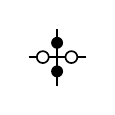
\begin{tikzpicture}[baseline={(0,-0.12)},x=1.2ex,y=1.2ex]%
        \draw [semithick] (-2, 0) to (2, 0);%
        \draw [semithick] (0, -2) to (0, 2);%
        \draw[semithick,fill=white] (-1, 0) circle(0.5ex);%
        \draw[semithick,fill=white] (1, 0) circle(0.5ex);%
        \fill[black] (0, 1) circle(0.5ex);%
        \fill[black] (0, -1) circle(0.5ex);%
    \end{tikzpicture}\kern-2pt\Big\rangle}

\newcommand{\SIbend}{\Big\lvert\kern0pt%
    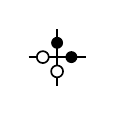
\begin{tikzpicture}[baseline={(0,-0.12)},x=1.2ex,y=1.2ex]%
        \draw [semithick] (-2, 0) to (2, 0);%
        \draw [semithick] (0, -2) to (0, 2);%
        \draw[semithick,fill=white] (-1, 0) circle(0.5ex);%
        \draw[semithick,fill=white] (0, -1) circle(0.5ex);%
        \fill[black] (0, 1) circle(0.5ex);%
        \fill[black] (1, 0) circle(0.5ex);%
    \end{tikzpicture}\kern-2pt\Big\rangle}

\newcommand{\SIstraightArrow}{\Big\lvert\kern0pt%
    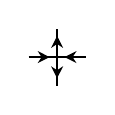
\begin{tikzpicture}[baseline={(0,-0.12)}]%
        \begin{scope}[semithick,decoration={
            markings,
            mark=at position 0.74 with {\arrow{Stealth[length=1.0ex,width=1.0ex]}}}
            ] 
            \draw[postaction={decorate}] (-2.4ex,0)--(0,0);
            \draw[postaction={decorate}] (2.4ex,0)--(0,0);
            \draw[postaction={decorate}] (0,0)--(0,2.4ex);
            \draw[postaction={decorate}] (0,0)--(0,-2.4ex);
        \end{scope}
    \end{tikzpicture}\kern-2pt\Big\rangle}

\newcommand{\SIbendArrow}{\Big\lvert\kern0pt%
    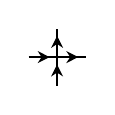
\begin{tikzpicture}[baseline={(0,-0.12)}]%
        \begin{scope}[semithick,decoration={
            markings,
            mark=at position 0.74 with {\arrow{Stealth[length=1.0ex,width=1.0ex]}}}
            ] 
            \draw[postaction={decorate}] (-2.4ex,0)--(0,0);
            \draw[postaction={decorate}] (0,0)--(2.4ex,0);
            \draw[postaction={decorate}] (0,0)--(0,2.4ex);
            \draw[postaction={decorate}] (0,-2.4ex)--(0,0);
        \end{scope}
    \end{tikzpicture}\kern-2pt\Big\rangle}

\newcommand{\clockwiseface}{\Big\lvert\kern0pt%
    
\begin{tikzpicture}[baseline={(0,-0.12)}]%
        \begin{scope}[semithick,decoration={
            markings,
            mark=at position 0.74 with {\arrow{Stealth[length=1.0ex,width=1.0ex]}}}
            ] 
            \draw[postaction={decorate}] (-1.2ex,1.2ex)--(1.2ex,1.2ex);
            \draw[postaction={decorate}] (1.2ex,1.2ex)--(1.2ex,-1.2ex);
            \draw[postaction={decorate}] (1.2ex,-1.2ex)--(-1.2ex,-1.2ex);
            \draw[postaction={decorate}] (-1.2ex,-1.2ex)--(-1.2ex,1.2ex);
        \end{scope}
    \end{tikzpicture}\kern-2pt\Big\rangle}

\newcommand{\anticlockwiseface}{\Big\lvert\kern0pt%
    
\begin{tikzpicture}[baseline={(0,-0.12)}]%
        \begin{scope}[semithick,decoration={
            markings,
            mark=at position 0.74 with {\arrow{Stealth[length=1.0ex,width=1.0ex]}}}
            ] 
            \draw[postaction={decorate}] (1.2ex,1.2ex)--(-1.2ex,1.2ex);
            \draw[postaction={decorate}] (-1.2ex,1.2ex)--(-1.2ex,-1.2ex);
            \draw[postaction={decorate}] (-1.2ex,-1.2ex)--(1.2ex,-1.2ex);
            \draw[postaction={decorate}] (1.2ex,-1.2ex)--(1.2ex,1.2ex);
        \end{scope}
    \end{tikzpicture}\kern-2pt\Big\rangle}

\newcommand{\neutralpattern}{%

\begin{tikzpicture}[baseline={(0,-0.12)},x=1ex,y=1ex]%
    \redcirc{0.0}{0};%
    \greencirc{2.4}{0};%
    \bluecirc{2*2.4}{0};%
    \redcirc{3*2.4}{0};%
    \greencirc{4*2.4}{0};%
    \bluecirc{5*2.4}{0};%
    \end{tikzpicture}
}


%%%%%%%%%%%%%%%%%%%%%%%%%%%%%%%%%%%%%%%%%%%%%%%%%%%%%%%%%%%%%%%
%                       Other commands                        %
%%%%%%%%%%%%%%%%%%%%%%%%%%%%%%%%%%%%%%%%%%%%%%%%%%%%%%%%%%%%%%%


\newcommand{\halfcirc}[4]{%
    \fill[#3, xshift={#1 ex}, yshift={#2 ex}] (0,0) -- (90:0.5ex) arc (90:270:0.5ex) -- cycle;%
    \fill[#4, xshift={#1 ex}, yshift={#2 ex}] (0,0) -- (270:0.5ex) arc (270:450:0.5ex) -- cycle;%
    \draw [semithick, xshift={#1 ex}, yshift={#2 ex}] (0, 0) circle(0.5ex);%
}

\newcommand{\redcross}[3]{%
    \draw [thick, red, xshift={#1 ex}, yshift={#2 ex}] ({-#3/2}, {-#3/2})--({#3/2}, {#3/2});%
    \draw [thick, red, xshift={#1 ex}, yshift={#2 ex}] ({-#3/2}, {#3/2})--({#3/2}, {-#3/2});%
}

\newcommand{\fadeleft}[4]{% default semithick linewidth
    \path[left color=black,right color=white] ({#1}, {#2-0.3pt}) rectangle ({#3}, {#4+0.3pt});
}
\newcommand{\faderight}[4]{% default semithick linewidth
    \path[left color=white,right color=black] ({#1}, {#2-0.3pt}) rectangle ({#3}, {#4+0.3pt});
}
\newcommand{\fadedown}[4]{% default semithick linewidth
    \path[top color=black,bottom color=white] ({#1-0.3pt}, {#2}) rectangle ({#3+0.3pt}, {#4});
}
\newcommand{\fadevertical}[6]{% default semithick linewidth
    \path[#1 color=black,#2 color=white] ({#3-0.3pt}, {#4}) rectangle ({#5+0.3pt}, {#6});
}
\newcommand{\fadehorizontal}[6]{% default semithick linewidth
    \path[#1 color=black,#2 color=white] ({#3}, {#4-0.3pt}) rectangle ({#5}, {#6+0.3pt});
}